\pstart\noindent\hangindent=10mm [17 v\textsuperscript{o}] (2) ex rotis\protect\index{Sachverzeichnis}{rota} decadicis, quibus conversiones \edlabel{num1start}\edtext{numerantur}{{\xxref{num1start}{num1end}}\lemma{}\Afootnote{numerantur. \textbar\ Harum commodissima ratio haec mihi videtur \textit{ (1) }\ , ut  Trochleae\protect\index{Sachverzeichnis}{trochlea|textit} sibi applicentur \textit{ (2) }\  ad praesens institutum quae aspicitur in adjecta figura, ubi si rota circumagitur vicibus 1000 rota \textit{b} eodem tempore circumagitur  \textit{(a)}\ semel, et rota\protect\index{Sachverzeichnis}{rota|textit} \textit{c} \textit{(b)}\ vicibus 100, et rota \textit{c} vicibus 10, et rota \textit{d} una vice. Ponamus rotae  \textbar\ primariae \textit{ erg.}\ \textbar\ conversiones esse  \textit{(aa)}\ 4 3 2 1, apparebit  numerus 1 in rota\protect\index{Sachverzeichnis}{rota|textit} \textit{a} numerus 2 in rota\protect\index{Sachverzeichnis}{rota|textit} \textit{b} numerus 3 in rota\protect\index{Sachverzeichnis}{rota|textit} \textit{c} \textit{(bb)}\ 9 6 4 1 apparebunt $\protect\begin{array}{lcccc} in\:rotis &a&b&c&d \\numeri&1&4&6&9\protect\end{array}$ \textit{ gestr.}\ \textbar\ (3) \textit{ L}}}.\pend
   %\begin{wrapfigure}{l}{0.25\textwidth}      
   \protect\begin{center}              
   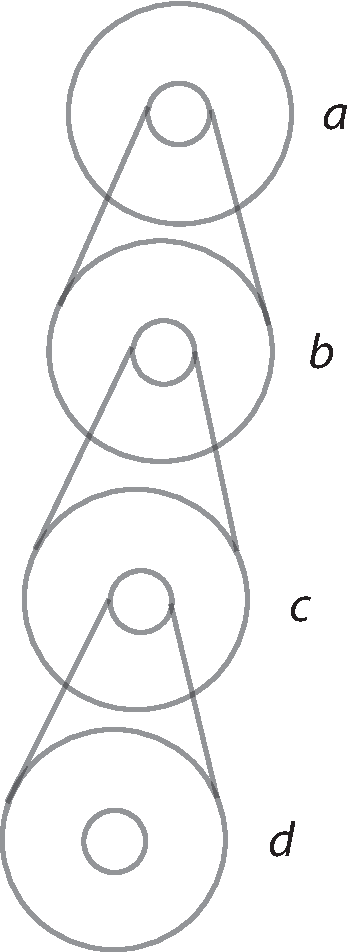
\includegraphics[width=0.2\textwidth]{images/38_17v}
   \\ \textit{[Fig. 1, gestr., tlw. Blindzeichnung]}\\
   \vspace{1.0ex}
   \protect\end{center}
 \clearpage
 \pstart\noindent\hangindent=10mm (3)\edlabel{num1end} ex mappa mobili, quae ad singulas 1000 (aut 100) ut lubet rotae\protect\index{Sachverzeichnis}{rota} \edtext{primariae}{\lemma{}\Afootnote{primariae \textit{ erg.} \textit{ L}}} conversiones amovetur  seu progreditur, cylindro involvente  veterem, evolvente novam, \pend
\pstart\noindent\hangindent=10mm (4) ex stylo ab acu magnetica\protect\index{Sachverzeichnis}{acus!magnetica} dependente,  qui ductus faciat in mappa subjacente, tum  rectos, \edtext{tum}{\lemma{rectos,}\Afootnote{ \textit{ (1) }\ seu \textit{ (2) }\ tum \textit{ L}}} curvos. \pend
\pstart\noindent\hangindent=20mm\hspace{20mm}Rectos, cum mappa \edtext{subjacens}{\lemma{}\Afootnote{subjacens \textit{ erg.} \textit{ L}}} ob revolutiones progreditur. \newline Curvos, cum ad sensum acus\protect\index{Sachverzeichnis}{acus!magnetica}, manente mappa, \edtext{converti videtur reapse mappa cum navi manente seu  directionem retinente acu, se \edlabel{convertitstart}convertit}{\lemma{mappa,}\Afootnote{ \textit{ (1) }\ reapse mappa (ob flexum navis\protect\index{Sachverzeichnis}{navis|textit}, quae  acu priorem directionem retinente se  convertit) \textit{ (2) }\ converti [...] convertit \textit{ L}}}. \pend \pstart\noindent\hangindent=30mm\hspace{30mm}\edtext{Illi\edlabel{convertitend}}{{\xxref{convertitstart}{convertitend}}\lemma{convertit.}\Afootnote{ \textit{ (1) }\  Recti \textit{ (2) }\   Illi \textit{ L}}} designant lineas  hi angulos cursus navis\protect\index{Sachverzeichnis}{navis}, seu lineae  motus. \pend \vspace{2.0ex}\pstart\begin{center}Difficultates seu objectiones \end{center}\pend \vspace{1.0ex}
\pstart\noindent\hangindent=10mm (1) non satis accurata erit delineatio, quia pyxis nautica\protect\index{Sachverzeichnis}{pyxis!nautica} non potest esse in satis multas partes divisa. \pend
\pstart\noindent\hangindent=20mm\hspace{20mm}Pyxidem\protect\index{Sachverzeichnis}{pyxis} enim parvam esse necesse est, alioqui \edtext{stylus}{\lemma{alioqui}\Afootnote{ \textit{ (1) }\ acus \textit{ (2) }\ stylus \textit{ L}}} \edtext{ductoris}{\lemma{}\Afootnote{ductoris \textit{ erg.} \textit{ L}}}, quippe a centro valde remotus, nimis ponderabit nec satis virium in acu\protect\index{Sachverzeichnis}{acus!magnetica} erit ad eum circumagendum \pend
\pstart\noindent\hangindent=10mm (2) ad ductus imprimendos vi quadam styli opus  est. Acus autem magnetica\protect\index{Sachverzeichnis}{acus!magnetica} est debilis \pend
\pstart\noindent\hangindent=10mm (3) jactatione navis\protect\index{Sachverzeichnis}{navis} \edtext{jactabitur}{\lemma{navis}\Afootnote{ \textit{ (1) }\ per \textit{ (2) }\ jactabitur \textit{ L}}} et pyxis\protect\index{Sachverzeichnis}{pyxis}, ac proinde ductus perturbabuntur \pend \pstart\noindent\hangindent=10mm (4) declinationes\protect\index{Sachverzeichnis}{declinatio} magneticae exactam cursus  delineationem impedient. \pend \vspace{2.0ex}